%% ----------------------------------------------------------------
%% Project.tex
%% ---------------------------------------------------------------- 
\documentclass[sotoncolour]{extra/uosproject}     % Use the Project Style with custom link colour
\usepackage[round]{natbib}     % Use Natbib style for the refs.
\usepackage{bibentry}          % Use bibentry for prepublished works
\usepackage{pdfpages}          % Enables PDF to be inserted into the project
\nobibliography*               % Use bibentry for prepublished works
\usepackage{attrib}            % Use the attrib package for quotations
\usepackage{}
\hypersetup{colorlinks=true}   % Set to false for black/white printing
%% ----------------------------------------------------------------
%% Definitions.tex
%% ---------------------------------------------------------------- 
\newcommand{\BibTeX}{{\rm B\kern-.05em{\sc i\kern-.025em b}\kern-.08em T\kern-.1667em\lower.7ex\hbox{E}\kern-.125emX}}

%% People
\newcounter{address}
\setcounter{address}{1}
\renewcommand{\theaddress}{\textsuperscript{\fnsymbol{address}}}
\newcommand{\address}[1]{\refstepcounter{address}\theaddress#1\\}
\newcommand{\Name}[3]{\texorpdfstring{\href{mailto:#3}{#2}#1}{#2}\xspace}
\newcommand{\SteveRGunn}[1]{\Name{#1}{Steve R. Gunn}{S.R.Gunn@ecs.soton.ac.uk}}

%% Dingbats
\newcommand{\tick}{\ding{51}}
\newcommand{\cross}{\ding{55}}

%% Calculus
\newcommand{\pd}[2]{\ensuremath{\frac{\partial #1}{\partial #2}}\xspace}
\newcommand{\fd}[2]{\ensuremath{\frac{d #1}{d #2}}\xspace}
\newcommand{\dint}{\ensuremath{\int\!\!\!\int}\xspace}
\newcommand{\tint}{\ensuremath{\int\!\!\!\int\!\!\!\int}\xspace}

%% Math Sets
\newcommand{\Q}[1]{\ensuremath{\mathbb{#1}}\xspace}
\newcommand{\R}{\Q{R}}

%% Matrix, Vector
\newcommand{\V}[1]{\ensuremath{\boldsymbol{#1}}\xspace}
\newcommand{\M}[1]{\ensuremath{\boldsymbol{#1}}\xspace}
\newcommand{\0}{\V{0}}
\newcommand{\1}{\V{1}}
\newcommand{\I}{\M{I}}

%% Math Functions
\newcommand{\F}[1]{\ensuremath{\mathrm{#1}}\xspace}
\newcommand{\sgn}{\F{sgn}}
\newcommand{\tr}{\F{trace}}
\newcommand{\diag}{\F{diag}}

%% Math Names
\newcommand{\N}[1]{\ensuremath{\mathit{#1}}\xspace}

%% Data
\newcommand{\mc}[1]{\ensuremath{\mathcal{#1}}\xspace}
\newcommand{\Hyp}{\mc{H}}
\newcommand{\D}{\mc{D}}

%% Kernel
\newcommand{\K}{\M{K}}
\newcommand{\eins}{\texorpdfstring{\ensuremath{\epsilon}}{\textepsilon}-insensitive\xspace}
\newcommand{\e}{\ensuremath{\epsilon}\xspace}
\newcommand{\Bxi}{\ensuremath{\boldsymbol{\xi}}\xspace}
\newcommand{\Kanova}{\ensuremath{\mathit{K_{ANOVA}}}\xspace}
\newcommand{\Kspline}{\ensuremath{\mathit{K_{spline}}}\xspace}

%% Bayesian
\newcommand{\MP}{\ensuremath{\mathit{{\scriptscriptstyle \hspace{-1.5pt}M\hspace{-1.5pt}P}}}\xspace}
\newcommand{\ML}{\ensuremath{\mathit{{\scriptscriptstyle \hspace{-1.5pt}M\hspace{-1.5pt}L}}}\xspace}
\newcommand{\Qw}{\ensuremath{Q_{\w}(\w)}\xspace}
\newcommand{\Qa}{\ensuremath{Q_{\Ba}(\Ba)}\xspace}
\newcommand{\Qb}{\ensuremath{Q_{\beta}(\beta)}\xspace}
\newcommand{\wMPab}{\ensuremath{\w_{\MP|\bar {\Ba},\bar \beta}}\xspace}
\newcommand{\wMP}{\ensuremath{\w_{\MP}}\xspace}
\newcommand{\yMP}{\ensuremath{y_{\MP}}\xspace}
\newcommand{\BaMP}{\ensuremath{\Ba_{\hspace{1pt}\MP}}\xspace}
\newcommand{\aMP}{\ensuremath{\alpha_{\hspace{1pt}\MP}}\xspace}
\newcommand{\bMP}{\ensuremath{\beta_{\hspace{1pt}\MP}}\xspace}
\newcommand{\Sab}{\ensuremath{\M{\Sigma}_{\bar \Ba,\bar \beta}}\xspace}
\newcommand{\Ba}{\ensuremath{\boldsymbol{\alpha}}\xspace}
\newcommand{\Bb}{\ensuremath{\boldsymbol{\beta}}\xspace}
\newcommand{\Bm}{\ensuremath{\boldsymbol{\mu}}\xspace}
\newcommand{\BL}{\ensuremath{\boldsymbol{\Lambda}}\xspace}
\newcommand{\BPhi}{\ensuremath{\boldsymbol{\Phi}}\xspace}
\newcommand{\SMP}{\ensuremath{\M{\Sigma}_{\MP}}\xspace}

\newcommand{\Pa}{\ensuremath{P(\alpha|\mathcal{H})}\xspace}
\newcommand{\Pb}{\ensuremath{P(\beta|\mathcal{H})}\xspace}
\newcommand{\Pab}{\ensuremath{P(\alpha,\beta|\mathcal{H})}\xspace}
\newcommand{\Pw}{\ensuremath{P(\w|\mathcal{H})}\xspace}
\newcommand{\PD}{\ensuremath{P(\D|\mathcal{H})}\xspace}
\newcommand{\PwIa}{\ensuremath{P(\w|\alpha,\mathcal{H})}\xspace}
\newcommand{\PDIwb}{\ensuremath{P(\D|\w,\beta,\mathcal{H})}\xspace}
\newcommand{\PDwab}{\ensuremath{P(\D,\w,\alpha,\beta|\mathcal{H})}\xspace}
\newcommand{\PDIw}{\ensuremath{P(\D|\w,\mathcal{H})}\xspace}
\newcommand{\PwID}{\ensuremath{P(\w|\D,\mathcal{H})}\xspace}
\newcommand{\PwabID}{\ensuremath{P(\w,\alpha,\beta|\D,\mathcal{H})}\xspace}

\newcommand{\PanH}{\ensuremath{P(\alpha)}\xspace}
\newcommand{\PbnH}{\ensuremath{P(\beta)}\xspace}
\newcommand{\PabnH}{\ensuremath{P(\alpha,\beta)}\xspace}
\newcommand{\PwnH}{\ensuremath{P(\w)}\xspace}
\newcommand{\PDnH}{\ensuremath{P(\D)}\xspace}
\newcommand{\PwIanH}{\ensuremath{P(\w|\alpha)}\xspace}
\newcommand{\PDIwbnH}{\ensuremath{P(\D|\w,\beta)}\xspace}
\newcommand{\PDwabnH}{\ensuremath{P(\D,\w,\Ba,\beta)}\xspace}
\newcommand{\PDIwnH}{\ensuremath{P(\D|\w)}\xspace}
\newcommand{\PwIDnH}{\ensuremath{P(\w|\D)}\xspace}
\newcommand{\PwabIDnH}{\ensuremath{P(\w,\alpha,\beta|\D)}\xspace}

\newcommand{\PDwBab}{\ensuremath{P(\D,\w,\Ba,\beta|\mathcal{H})}\xspace}
\newcommand{\PwIBa}{\ensuremath{P(\w|\Ba,\mathcal{H})}\xspace}
\newcommand{\PBab}{\ensuremath{P(\Ba,\beta|\mathcal{H})}\xspace}
\newcommand{\PwBabID}{\ensuremath{P(\w,\Ba,\beta|\D,\mathcal{H})}\xspace}

\newcommand{\PBanH}{\ensuremath{P(\Ba)}\xspace}
\newcommand{\PwIBanH}{\ensuremath{P(\w|\Ba)}\xspace}

%% Snakes
\newcommand{\Esnake}{\ensuremath{\mathit{E_{snake}}}\xspace}
\newcommand{\Eimage}{\ensuremath{\mathit{E_{image}}}\xspace}
\newcommand{\Econt}{\ensuremath{\mathit{E_{cont}}}\xspace}
\newcommand{\Ecurv}{\ensuremath{\mathit{E_{curv}}}\xspace}
\newcommand{\Eint}{\ensuremath{\mathit{E_{int}}}\xspace}
\newcommand{\Eext}{\ensuremath{\mathit{E_{ext}}}\xspace}
\newcommand{\Eterm}{\ensuremath{\mathit{E_{term}}}\xspace}
\newcommand{\Eline}{\ensuremath{\mathit{E_{line}}}\xspace}
\newcommand{\Eedge}{\ensuremath{\mathit{E_{edge}}}\xspace}
\newcommand{\Econ}{\ensuremath{\mathit{E_{con}}}\xspace}
\newcommand{\Eangle}{\ensuremath{\mathit{E_{angle}}}\xspace}
\newcommand{\Elshape}{\ensuremath{\mathit{E_{lshape}}}\xspace}
\newcommand{\Eedgedir}{\ensuremath{\mathit{E_{edgedir}}}\xspace}
\newcommand{\Emodel}{\ensuremath{\mathit{E_{model}}}\xspace}
\newcommand{\wte}{\ensuremath{\mathit{w_{term}}}\xspace}
\newcommand{\wli}{\ensuremath{\mathit{w_{line}}}\xspace}
\newcommand{\wed}{\ensuremath{\mathit{w_{edge}}}\xspace}
\newcommand{\wco}{\ensuremath{\mathit{w_{con}}}\xspace}

%% Environments
\newcounter{alg}
\newenvironment{algorithm}[1]
{
    \stepcounter{alg}
    \begin{table}[htb]
    \centering
    \begin{tabular}[t]{ll}
    \hline&\\
    \multicolumn{2}{l}{\bf Algorithm \arabic{alg}: #1}\\&\\
} {
    &\\
    \hline
    \end{tabular}
    \end{table}
}
      % Include your abbreviations

%% ----------------------------------------------------------------
%% --------------------THESIS/DOC INFORMATION ---------------------
\department  {School of Electronics and Computer Science}
\DEPARTMENT  {\MakeUppercase{\deptname}}
\group       {}
\GROUP       {\MakeUppercase{\groupname}}
\faculty     {Faculty of Physical Engineering and Science}
\FACULTY     {\MakeUppercase{\facname}}
\title       {Auctions for online elastic resource allocation in cloud computing}
\authors     {\texorpdfstring
             {\href{mailto:mt5g17@soton.ac.uk}{Mark Towers}}
             {Mark Towers}}
\addresses  {\groupname\\\deptname\\\univname}
\date       {\today}
\supervisor {Dr Tim Norman}
\examiner   {}
\degree     {MEng Electronic Engineering}
%% Optional Fields TODO: Replace these fields with your own data
\qualifications{}
\subject    {}
\keywords   {Auctions, reinforcement learning, cloud computing}

\begin{document}
%% ------------------ FRONT MATTER ORGANISATION -------------------
\frontmatter
\maketitle
\begin{abstract}
Edge clouds enable computational tasks to be completed at the edge of the network, without relying on access to remote data centres. A key challenge in these settings is that limited computational resources often need to be allocated to many self-interested users. Here, existing resource allocation approaches usually assume that tasks have inelastic resource requirements (i.e., a fixed amount of compute time, bandwidth and storage), which may result in inefficient resource use. In this paper, we expand previous work to an online setting such that job will arrive over time with the task prices and resource allocation determined through training an agent using reinforcement learning.  
\end{abstract}
\pdfbookmark[0]{\contentsname}{toc}
\tableofcontents
% \listoffigures
% \listoftables
%% The List of listings does not, by default, appear in the ToC, so....
\addtotoc{Listings}
% \lstlistoflistings
% \listofaddmaterial
% \addtolom{Material Name e.g Map}
% \addtolom{Material Name e.g CD}
% \addtolom{Test Material}
%% ---------- AUTHORSHIP DECLARATION/ ACKNOW. / DEDICATORY ----------
%% Either include citations like below (as many as required spaced with commas or 'and').
%% \bibentry command must be used here with prepublished papers
\authorshipdeclaration{\bibentry{Gunn:2001:pdflatex}\newline\bibentry{Lovell:2011:updated}\newline\bibentry{Gunn:2011:updated2}}
%% Or state no citations like below
%% \authorshipdeclaration{}
%% -----------------------
\acknowledgements{
This project wouldn't have started without Dr Sebastian Stein and a team of Pennsylvania State University that has produced a paper investigating the static case of this problem. So I am grateful for the support they gave in kick starting this project.\\ Also to my housemate for surviving with me pestering them about proof reading my paper and this project all of the time.}

% \dedicatory{To \dots}
%%Lightweight Definitions and Abbreviations see package:nomencl for alternative
%% Include if relevant to discipline
% \listofsymbols{ll}{$w$ & The weight vector\\$\S$ & If relevant to discipline}

% Todo citep insteads of cite for adding brackets around the citation
\mainmatter
%% ------------------ MAIN MATTER (CONTENT) --------------------
\chapter{Introduction}
When computer programs are too large, difficult or time consuming to be run on a normal computer, these programs are often offloaded to cloud providers like Google Cloud Platform, Amazon Web Service, Microsoft Azure and many more. These providers all allow customers to individually request a set of resources to compute their program with. However, this can create a bottleneck on certain resource preventing other jobs from running with this fixed requirement model. This project considers the case where users don't request a set amount of resources but rather the user details the total requirements for the program and a deadline for when the program must be finished. This then means that the cloud provider can effectively balances resource demands as it has complete knowledge of its different user's requirements, allowing more jobs to run simultaneously and lower price as there can be a lower overall demand of individual resources. 

In the last few years, cloud computing~\cite{cloud_cite} has become a popular solution to run data-intensive applications remotely. However, in some application domains, it is not feasible to rely a remote cloud, for example when running highly delay-sensitive and computationally-intensive tasks, or when connectivity to the cloud is intermittent. To deal with such domains, \emph{mobile edge computing}~\cite{mobile_edge_survey} has emerged as a complementary paradigm, where computational tasks are executed at the edge of mobile networks at small data-centers, known as \emph{edge clouds}.

Mobile edge computing is a key enabling technology for the Internet-of-Things (IoT) \cite{mobile_edge_IoT} and in particular applications in smart cities \cite{mobile_edge_smart} and disaster response scenarios \cite{mobile_edge_disaster}. In these applications, low-powered devices generate computational tasks and data that have to be processed quickly on local edge cloud servers. More specifically, in smart cities, these devices could be smart intersections that collect data from road-side sensors and vehicles to produce an efficient traffic light sequence to minimize waiting times \cite{smart_cities_traffic_lights}; or it could be CCTV cameras that analyse video feeds for suspicious behaviour, e.g., to detect a stabbing or other crime in progress \cite{Sreenu2019}. In disaster response, sensor data from autonomous vehicles (including video, sonar and LIDAR) can be aggregated in real time to produce maps of a devastated area, search for potential victims and help first responders in focusing their efforts to save lives \cite{smart_disaster_management}.

To accomplish these tasks, there are typically several types of resources that are needed, including communication bandwidth, computational power and data storage resources \cite{vaji_infocom}, and tasks are generally delay-sensitive, i.e., have a specific completion deadline. When accomplished, different tasks carry different values for their owners (e.g., the users of IoT devices or other stakeholders such as the police or traffic authority). This value will depend on the importance of the task, e.g., analysing current levels of air pollution may be less important than preventing a large-scale traffic jam at peak times or tracking a terrorist on the run. Given that edge clouds are often highly constrained in their resources \cite{edge_limitations}, we are interested in allocating tasks to edge cloud servers to maximize the overall social welfare achieved (i.e., the sum of all task values). This is particularly challenging, because users in edge clouds are typically self-interested and may behave strategically \cite{Bi2019} or may prefer not to reveal private information about their values to a central allocation mechanism \cite{Pai2013}.

An important shortcoming of existing work looking at resource allocation in edge clouds, e.g., \cite{vaji_infocom,Bi2019}, is that it assumes tasks have strict resource requirements --- that is, each task consumes a fixed amount of computation (CPU cycles per time), takes up a fixed amount of bandwidth to transfer data and uses up a fixed amount of storage on the server. However, in practice, edge cloud servers have some flexibility in how they allocate limited resources to each task. In more detail, to execute a task, the corresponding data and/or code first has to be transferred to the server it is assigned to, requiring some bandwidth. This then takes up storage on the server. Next, the task needs computing power from the server in terms of CPU cycles per time. Once computation is complete, the results have to be transferred back to the user, requiring further bandwidth. Now, while the the storage capacity at the server for every task is \emph{strict}, since the task cannot be run unless all the data are stored, the bandwidth allocation and the speed at which the task is run on the server are \emph{elastic}. The latter two depend on how tight the task's deadline is, and can be adjusted  accordingly, so that more tasks can receive service simultaneously. Allocating the elastic resources optimally is the focus of this paper where job may be arriving over time such for that server can redistribute their resource as new resources arrive.

\chapter{Related Works}
There is a considerable amount of research in the area of resource allocation and pricing in cloud computing, some of which use auction mechanisms to deal with competition~\cite{KUMAR2017234,Zhang2017,Du2019,Bi2019}. % Put a couple of more references. 
However, a majority of these approaches assume that users request a fixed amount of resources system resources and processing rates, with the cloud provider having no control over the speeds, only the servers that the task was allocated to.  In our work and appendix \ref{app:aamas_paper}, tasks' owners report deadlines and overall data and computation requirements, allowing the edge cloud server to distribute its resources more efficiently based on each task's requirements. But the appendix \ref{app:aamas_paper} considers the case where all jobs arrive at the same time whereas this project considers the case of tasks arriving overtime. 

Other closely related work on resource allocation in edge clouds \cite{vaji_infocom} considers both the placement of code/data needed to run a specific task, as well as the scheduling of tasks to different edge clouds. The goal there is to maximize the expected rate of successfully accomplished tasks over time. Our work is different both in the setup and the objective function. Our objective is to maximize the value over all tasks. In terms of the setup, they assume that data/code can be shared and they do not consider the elasticity of resources.

Reinforcement learning has a huge amount of research \cite{Sutton1998} allowing for an agent to be trained by engaging with an environment that receives reward from taking certain actions. As our environment has action that affect the environment and future actions, supervised and unsupervised learning are not able to be used to train the agent. This has primarily been used in games \cite{atari, silver2017mastering} as it allows for agent to interact with the environment with an affect the environment which results in a reward. As our problem case allows the agent to interact with the environment that results in rewards from the actions it takes meaning that the agent can discover the best strategies for bidding and allocating resources instead of using heuristics predetermined by a human. 

\chapter{Proposed solution}\label{sec:proposed_solution}
As the problem case has two stage that must be consider: the bidding of available jobs and the allocation of resource for allocated jobs. Due to each of these stages requiring and returning different variables, two different function approximation will be found, discussed in sections \ref{subsec:auction_solution} and \ref{subsec:resource_allocation} respectively.

\begin{figure}
    \centering
    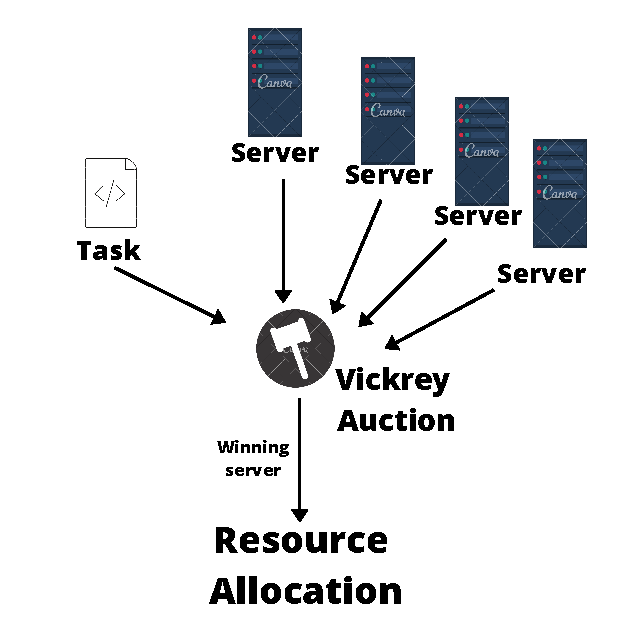
\includegraphics{extra/system_model.pdf}
    \caption{System model}
    \label{fig:system_model}
\end{figure}

A sketch of the system is shown in Fig.~\ref{fig:system_model}. 
We assume that in the system there is a set of servers $I = \{1,2,\ldots,\left|I\right|\}$ servers, which could be edge clouds that can be accessed either through cellular base stations or WiFi access points (APs). Servers have different types of resources: storage for the code/data needed to run a task (e.g., measured in GB), computation capacity in terms of CPU cycles per time interval (e.g., measured in FLOP/s), and communication bandwidth to receive the data and to send back the results of the task after execution (e.g., measured in Mbit/s). We assume that the servers are heterogeneous in all their characteristics. More formally, we denote the storage capacity of server $i$ with $S_i$, computation capacity with $W_i$, and the communication capacity with $R_i$.

There is a set $J = \{1,2,\ldots,\left| J \right|\}$ of  different tasks that require service from one of the servers in set $I = \{1,2,\ldots, \left| I \right|\}$. To run any of these tasks on a server requires storing the appropriate code/data on the same server. These could be, for example, a set of images, videos or CNN layers in identification tasks. The storage size of task $j$ is denoted as $s_j$ with the rate at which the program is transferred to the server $i$ at time $t$ being $s^{'}_{i,j,t}$. For a task to be computed successfully, it must fetch and execute instructions on a CPU. We consider the total number of CPU cycles required for the program to be $w_j$, where the rate at which the CPU cycles are assigned to the task on server $i$ at time $t$ is $w^{'}_{i,j,t}$. Finally, after the task is run and the results obtained, the latter need to be sent back to the user. The size of the results for task $j$ is denoted with $r_j$, and the rate at which they are sent back to the user is $r^{'}_{i,j,t}$ on server $i$ at time $t$. Every task has a beginning time, denoted by $b_j$ and a deadline, denoted by $d_j$. This is the maximum time for the task to be completed in order for the user to derive its value. This time includes: the time required to send the data/code to the server, run it on the server, and get back the results. Therefore for the task to be successfully completed, it must completed fulfill the constraint in equation~\eqref{eq:deadline}. These operations must occur in order as a server couldn't compute a task that was not fully loaded on the machine therefore the whole of the loading stage must be completed before moving onto the compute stage and likewise for the sending of results. 

\begin{align}
    \frac{s_j}{\sum^{d_j}_{t=b_j} s^{'}_{i,j,t}} + \frac{w_j}{\sum^{d_j}_{t=b_j} w^{'}_{i,j,t}}  + \frac{r_j}{\sum^{d_j}_{t=b_j} r^{'}_{i,j,t}} \leq d_j && \forall{j \in J}  \label{eq:deadline}
\end{align}

As server have limited capacity, the total resource usages for all tasks running on a server must be capped to the resource capacity. The storage constraint (equation \eqref{eq:server_storage_capacity}) is unique as the previous amount loaded in kept till the end of a program on server. While the computation capacity (equation \eqref{eq:server_computation_capacity} is the sum of compute used by all of the tasks on a server and the bandwidth capacity (equation \eqref{eq:server_bandwidth_capacity}) is the sum of loading and sending usages by tasks. 
\begin{align}
    \sum_{j \in J} \left(\sum^{d_j}_{t=b_j} s^{'}_{i,j,t} \right) \leq S_i, && \forall{i \in I} \label{eq:server_storage_capacity} \\
    \sum_{j \in J} w^{'}_{i,j,t} \leq W_i, && \forall{i \in I, t \in T} \label{eq:server_computation_capacity} \\
    \sum_{j \in J} s^{'}_{i,j,t} + r^{'}_{i,j,t} \leq R_i, && \forall{i \in I, t \in T} \label{eq:server_bandwidth_capacity} \\
\end{align}

\section{Auction solution}\label{subsec:auction_solution}
If an agent wish to run on task on the cloud, the task can be put forward with its requirements of required storage, computation, results data and deadline. In order for fast and truthful, a reverse of the Vickrey auction (\cite{vickrey}) will be used as it is a second-price sealed-bid auction. Bidders all submit their bid for the task, that is a single indivisible item being sold, where all bidders are incentive to bid their true valuation as the winner with the lowest price actually pays the second lowest price. Making truthful bidding the dominant strategy for bidding on a task preventing the need for agent to learn how to outbid another agent as it only needs to consider its evaluation. As there is also only a single round of bidding compared to alternative auctions like English or Dutch auctions allowing fast auctioning of task no matter the number of possible servers and can be done in parallel with other jobs being allocated. % If to use a reserve price is unknown at this time

In order to calculate the price of the task for a server requires a understanding the resource requirements of the task, the future supply and demand for tasks and the resource requirements of currently allocated tasks. Due to the complexity in creating a heuristic that can accurately use this information and the amount of memory required for a table based approach. Therefore function approximator will be used to approximate the value of the task to the server with Long/Short Term Memory (LSTM) neural network~\cite{LSTM}. The justified for the use of this network over other models is explained in section~\ref{subsec:just_auction}. 

\section{Resource allocation solution}\label{subsec:resource_allocation}
In previous work (appendix \ref{app:aamas_paper}), that utilised a single shot problem case where jobs wouldnt arrive over time meant that resource speed had a fixed speed and assumed that a task loading, computing and sending result occurred concurrently. However due to the addition of time means that the task contains stages for the loading, computing and sending of results thus requiring for the resources allocated to a task must change over time. Therefore at each time step, a server needs to reallocate all of its resource to its currently allocated tasks as some tasks will have completely one of its stages. 

In order to select how to allocate resource to tasks, this problem doesn't seem as complex as the pricing in section \ref{subsec:auction_solution} therefore simple heuristic and long/short term memory neural network will be implemented. This is justified in section~\ref{subsec:just_resource_allocation}.

%\begin{table}[]
%    \centering
%    \begin{tabular}{|c|l|c|l} \hline
%     Decision Variable & Description \\ \hline \hline
%        
%        $s_j$ & Task $j$ storage requirements \\ \hline
%        $w_j$ & Task $j$ computation requirements \\ \hline
%        $r_j$ & Task $j$ results data requirements \\ \hline
%        $p_j$ & Task $j$ value (the price paid) \\ \hline
%        $c_j$ & Task $j$ start time \\ \hline
%        $d_j$ & Task $j$ deadline time \\ \hline \hline
%        
%        $S_i$ & Server $i$ storage capacity \\ \hline 
%       $W_i$ & Server $i$ computational capacity \\ \hline
%        $R_i$ & Server $i$ bandwidth capacity \\ \hline \hline
%        
%        $s^{'}_{i,j,t}$ & Task $j$ loading speed on server $i$ at time $t$ \\ \hline
%        $w^{'}_{i,j,t}$ & Task $j$ compute speed on server $i$ at time $t$ \\ \hline
%        $r^{'}_{i,j,t}$ & Task $j$ sending speed on server $i$ at time $t$ \\ \hline
%        
%        $\hat{s}_{i,j,t}$ & Task $j$ loading stage completion on server $i$ at time $t$ \\ \hline
%        $\hat{w}_{i,j,t}$ & Task $j$ computational stage completion on server $i$ at time $t$ \\ \hline
%        $\hat{r}_{i,j,t}$ & Task $j$ sending stage completion on server $i$ at time $t$ \\ \hline
%    \end{tabular}
%    \caption{Optimisation decision variables}
%    \label{tab:decision_var}
%\end{table}

%\begin{align}
%    max & \sum_{j \in J} p_j \sum_{i \in I} \hat{r}_{i,j,d_j} \\
%    \mbox{s.t.} \nonumber \\
%    & 0 \leq s^{'}_{i,j,t} \leq \infty, &~ \forall{i \in I, j \in J, t \in T} \label{eq:loading_speed_limits} \\ % Loading speed limits 
%    & 0 \leq w^{'}_{i,j,t} \leq \infty, &~ \forall{i \in I, j \in J, t \in T} \label{eq:compute_speed_limits} \\ % Compute speed limits
%    & 0 \leq r^{'}_{i,j,t} \leq \infty, &~ \forall{i \in I, j \in J, t \in T} \label{eq:sending_speed_limits} \\ % Sending speed limits
%    & \sum^{c_j - 1}_{t = 1} s^{'}_{i,j,t} = 0, &~ \forall{i \in I, j \in J} \label{eq:pre_loading_stage} \\ % Stops loading before start time
%    & w^{'}_{i,j,t} \leq \hat{s}_{i,j,t} \cdot w_j, &~ \forall{i \in I, j \in J, t \in T} \label{eq:pre_compute_stage} \\ % Stops computing before loading finished
%    & r^{'}_{i,j,t} \leq \hat{w}_{i,j,t} \cdot r_k, &~ \forall{i \in I, j \in J, t \in T} \label{eq:pre_sending_stage} \\ % Stops sending results before computation is finished
%    & \hat{s}_{i,j,t} \leq \frac{\sum^{t}_{t^{'} = 0} s^{'}_{i,j,t^{'}}}{S_j}, &~ \forall{i \in I, j \in J, t = 1,...,d_j} \label{eq:overload_loading_speed} \\
%    & \hat{s}_{i,j,t} = \lfloor \frac{\sum^{t}_{t^{'} = 0} s^{'}_{i,j,t^{'}}}{S_j} \rfloor, &~ \forall{i \in I, j \in J, t = 1,...,d_j} \label{eq:loading_speed_stage_completion} \\
%    & \hat{w}_{i,j,t} \leq \frac{\sum^{t}_{t^{'} = 0} w^{'}_{i,j,t^{'}}}{W_j}, &~ \forall{i \in I, j \in J, t = 1,...,d_j} \label{eq:overload_compute_speed} \\
%    & \hat{w}_{i,j,t} = \lfloor \frac{\sum^{t}_{t^{'} = 0} w^{'}_{i,j,t^{'}}}{W_j} \rfloor, &~ \forall{i \in I, j \in J, t = 1,...,d_j} \label{eq:compute_speed_stage_completion} \\
%    & \hat{r}_{i,j,t} \leq \frac{\sum^{t}_{t^{'} = 0} r^{'}_{i,j,t^{'}}}{R_j}, &~ \forall{i \in I, j \in J, t = 1,...,d_j} \label{eq:overload_sending_speed} \\
%    & \hat{r}_{i,j,t} = \lfloor \frac{\sum^{t}_{t^{'} = 0} r^{'}_{i,j,t^{'}}}{R_j} \rfloor, &~ \forall{i \in I, j \in J, t = 1,...,d_j} \label{eq:sending_speed_stage_completion} \\
%    & \sum_{j \in J} (\sum^{t}_{t^{'} = 0} s_{i,j,t^{'}}) \cdot \hat{r}_{i,j,t} \leq S_i, &~ \forall{i \in I, j \in J, t \in T} \label{eq:server_storage_capacity} \\
%    & \sum_{j \in J} w^{'}_{i,j,t} \leq W_i, &~ \forall{i \in I, j \in J, t \in T} \label{eq:server_computation_capacity} \\
%    & \sum_{j \in J} s^{'}_{i,j,t} + r^{'}_{i,j,t} \leq R_i, &~ \forall{i \in I, j \in J, t \in T} \label{eq:server_bandwidth_capacity} 
%\end{align}

\chapter{Justification of the approach}
The proposed solution in section \ref{sec:proposed_solution} has been chosen due to a variety of reasons. 

\section{Justification for the auction} \label{subsec:just_auction}
The vickrey auction (~\cite{vickrey}) has been chosen as it a dominant strategy for agents is to truthfully report the their true evaluation of a task to it. This project will require to reverse as it is the server are selling their resources and buying the tasks for a price with the lowest price winning instead of the standard pricing model where the highest price winning the item. However dispute this change of swapping the pricing model, the dominant strategy is truthful reporting as if server report negative prices for a task then the highest negative number is equal to the lowest positive number. 

\section{Justification for resource allocation} \label{subsec:just_resource_allocation}


\chapter{Work requirements}
An estimate of any support required to complete the project
* Only Iridis 4 with GPU (currently have access to Iridis 4)

\section{Work to date}
% include grantt chart
\begin{figure}
    \centering
    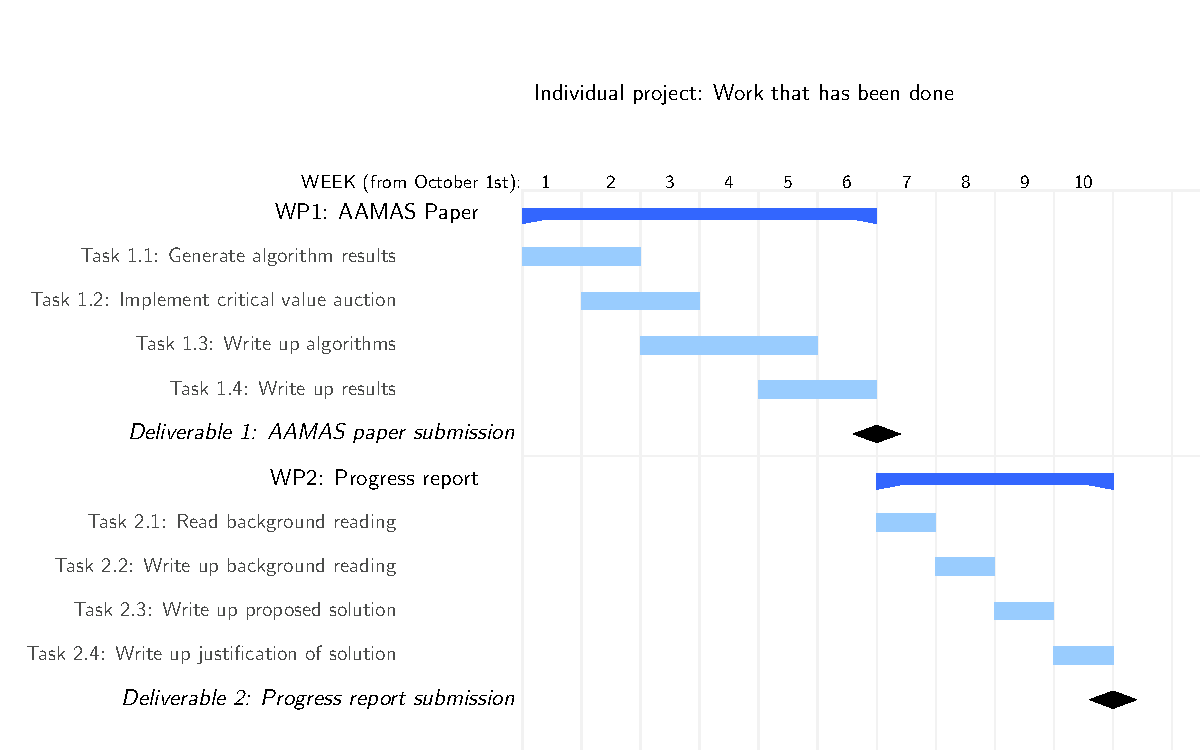
\includegraphics{past_work_grantt/past_grantt.pdf}
    \caption{Work that has been done to date}
    \label{fig:past_grantt}
\end{figure}

\section{Plan of the remaining work}
% include grantt chart
\begin{figure}
    \centering
    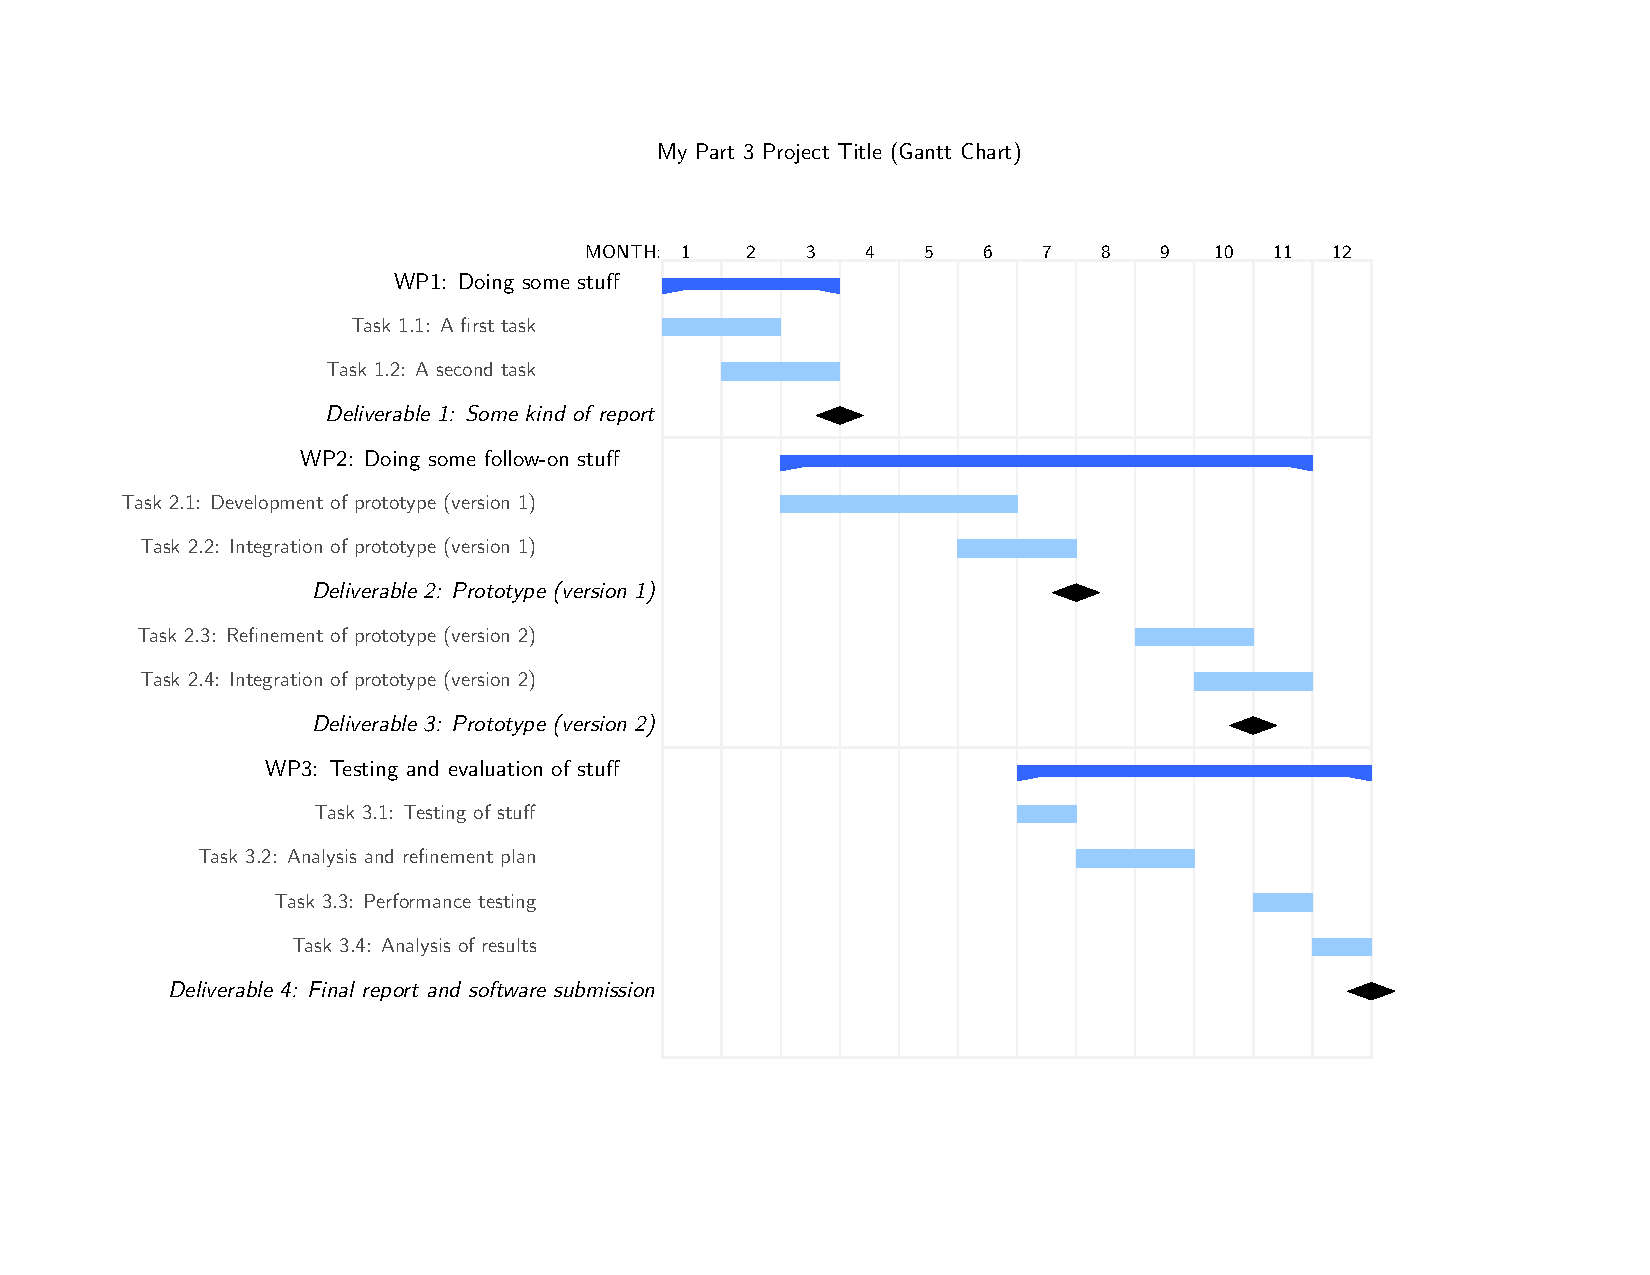
\includegraphics{future_work_grantt/future_grantt}
    \caption{}
    \label{fig:future_grantt}
\end{figure}

\backmatter

\appendix
\section*{Appendix A}\label{app:aamas_paper} % Insert the AAMAS paper
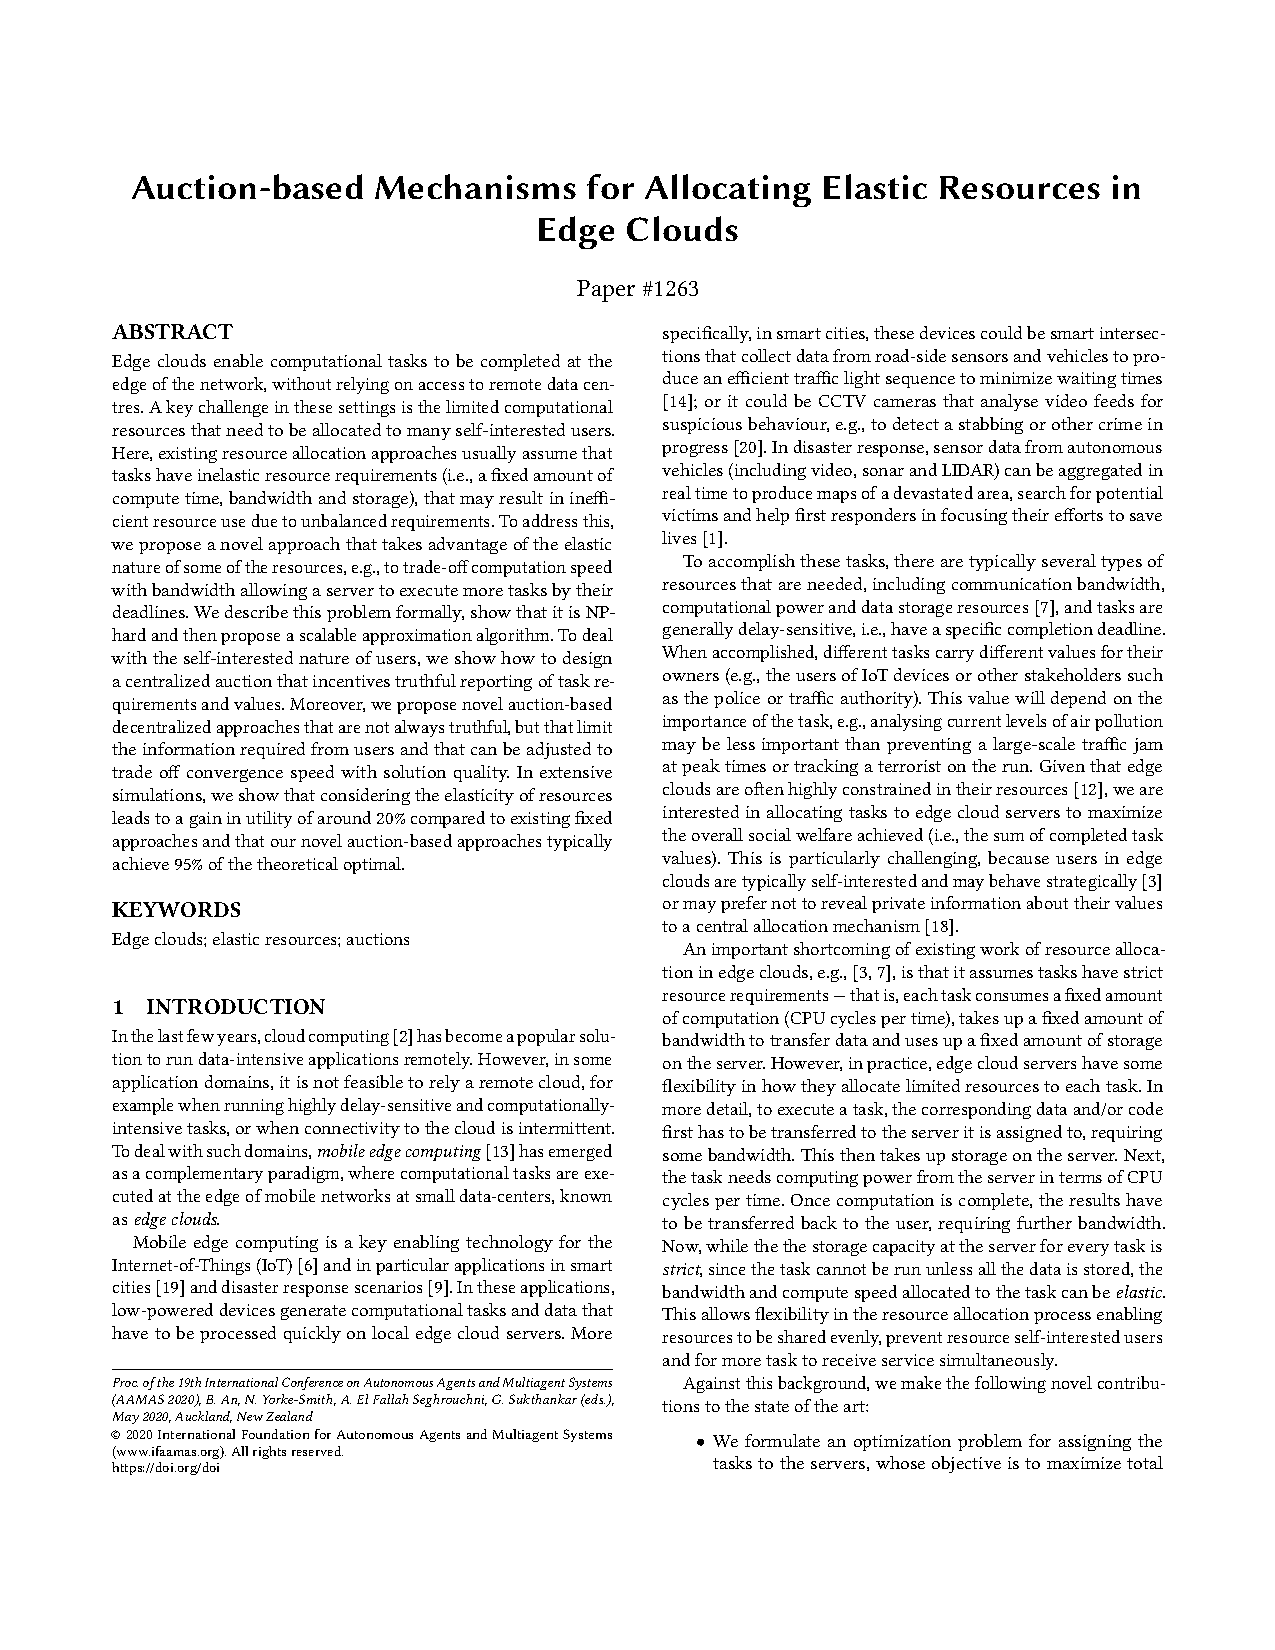
\includepdf[pages={1}, offset=-25mm -20mm]{extra/aamas_2020}
\includepdf[pages={2}, offset= 25mm -20mm]{extra/aamas_2020}
\includepdf[pages={3}, offset=-25mm -20mm]{extra/aamas_2020}
\includepdf[pages={4}, offset= 25mm -20mm]{extra/aamas_2020}
\includepdf[pages={5}, offset=-25mm -20mm]{extra/aamas_2020}
\includepdf[pages={6}, offset= 25mm -20mm]{extra/aamas_2020}
\includepdf[pages={7}, offset=-25mm -20mm]{extra/aamas_2020}
\includepdf[pages={8}, offset= 25mm -20mm]{extra/aamas_2020}

\bibliographystyle{plainnat}
\bibliography{extra/references}
\end{document}
%% ----------------------------------------------------------------
